
\documentclass{standalone}
\usepackage[svgnames]{xcolor}
\usepackage{pgfplots}
\pgfplotsset{compat=newest}
\usepackage[sfdefault]{FiraSans}
\usepackage{FiraMono}
\renewcommand*\familydefault{\sfdefault}
\begin{document}
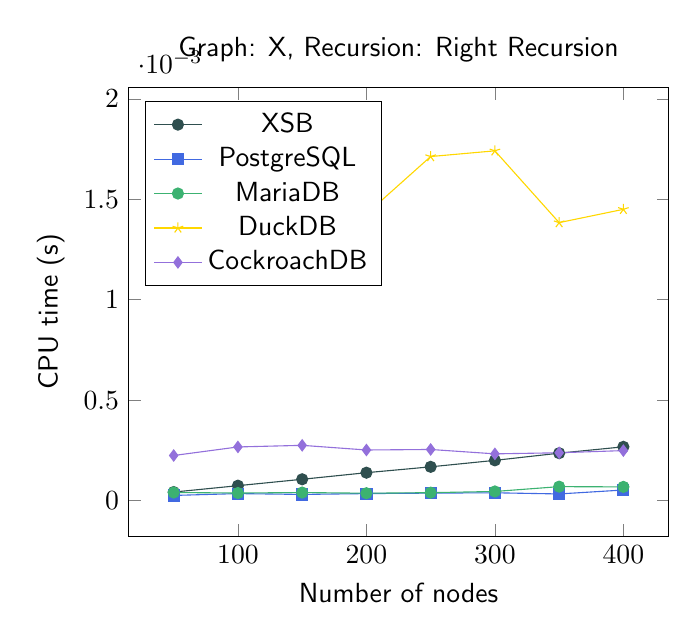
\begin{tikzpicture}
    \begin{axis}[
        title={Graph: X, Recursion: Right Recursion},
        xlabel={Number of nodes},
        ylabel={CPU time (s)},
        legend pos={north west},
        ymax=0.0020544000000000005
    ]
    \addplot+[DarkSlateGray, mark options={color=DarkSlateGray}] coordinates {(50,4.240000000000008e-05) (100,7.419999999999993e-05) (150,0.000106) (200,0.0001388000000000002) (250,0.00016800000000000002) (300,0.0002002000000000002) (350,0.00023600000000000018) (400,0.00026760000000000005)};
\addlegendentry{XSB}
\addplot+[RoyalBlue, mark options={color=RoyalBlue}] coordinates {(50,2.5600000000003397e-05) (100,3.4800000000012596e-05) (150,3.0599999999991745e-05) (200,3.4800000000012596e-05) (250,3.7200000000015e-05) (300,3.87999999999944e-05) (350,3.299999999999415e-05) (400,5.259999999999154e-05)};
\addlegendentry{PostgreSQL}
\addplot+[MediumSeaGreen, mark options={color=MediumSeaGreen}] coordinates {(50,4.0199999999990244e-05) (100,3.759999999998209e-05) (150,3.999999999998449e-05) (200,3.6599999999997745e-05) (250,3.9399999999989445e-05) (300,4.5399999999995445e-05) (350,6.939999999999724e-05) (400,6.820000000000715e-05)};
\addlegendentry{MariaDB}
\addplot+[Gold, mark options={color=Gold}] coordinates {(50,0.001108000000000009) (100,0.001206000000000007) (150,0.0015812000000000048) (200,0.0014270000000000116) (250,0.0017126000000000196) (300,0.0017410000000000036) (350,0.001383600000000007) (400,0.0014498000000000121)};
\addlegendentry{DuckDB}
\addplot+[MediumPurple, mark options={color=MediumPurple}] coordinates {(50,0.00022440000000000236) (100,0.000266999999999995) (150,0.000275000000000003) (200,0.00025179999999999094) (250,0.0002543999999999991) (300,0.00023260000000000503) (350,0.00023799999999999378) (400,0.00024879999999999347)};
\addlegendentry{CockroachDB}

    \end{axis}
\end{tikzpicture}
\end{document}
